\section{Oszilatoren}
\subsection{Typen}
	\begin{center}
		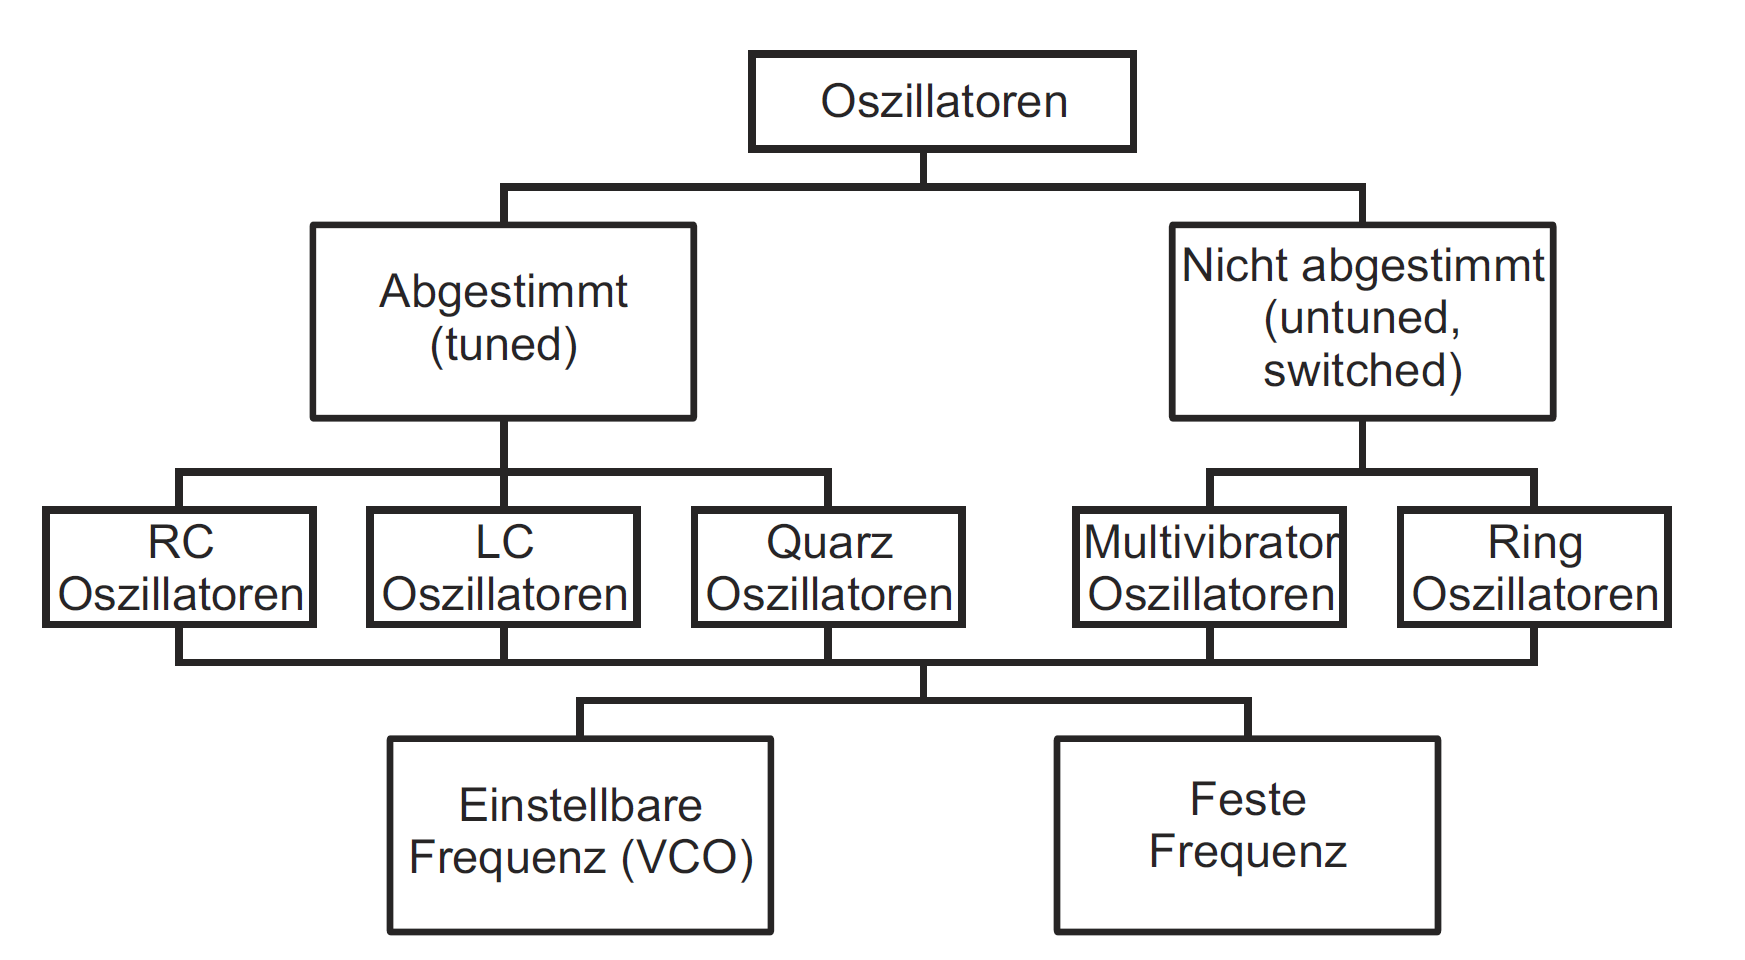
\includegraphics[width=11cm]{bilder/osziTypen.png}
	\end{center}
\subsection{Rechteckgenerator}
	\begin{multicols}{3}
		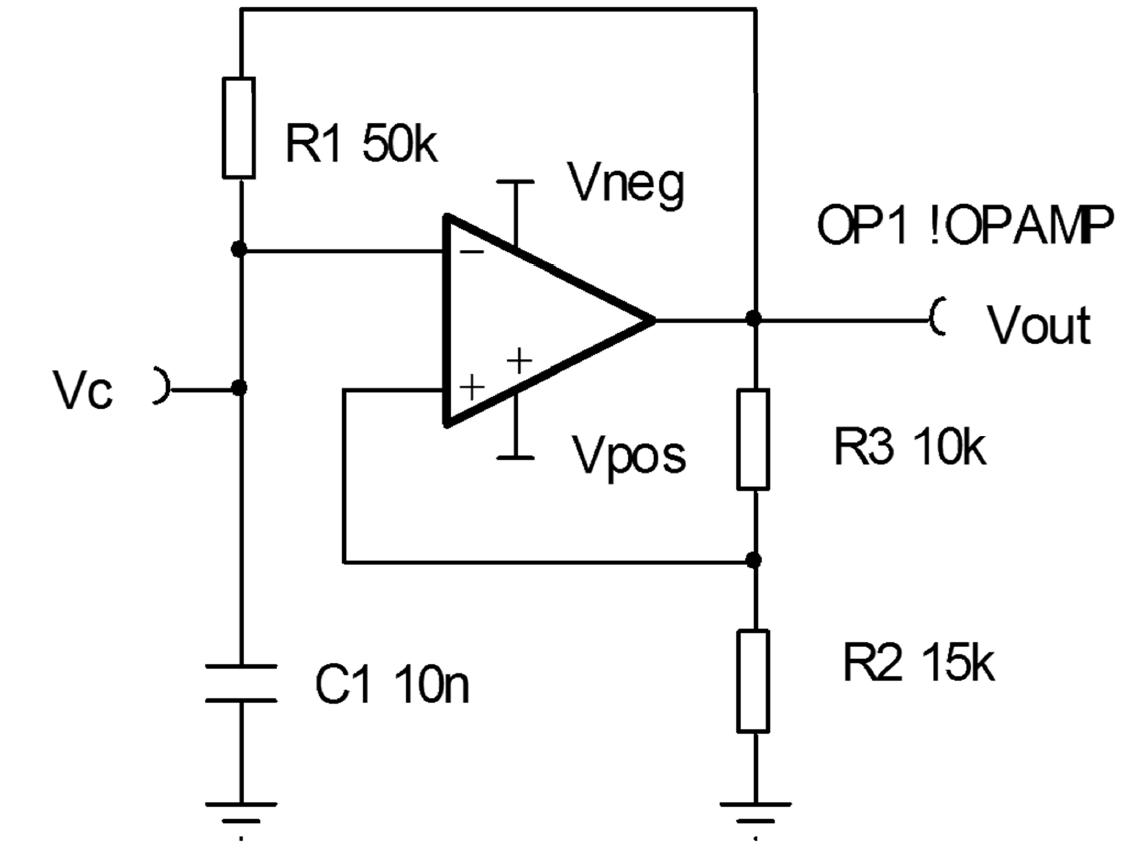
\includegraphics[width=6cm]{bilder/osziRechteck.png}
		\columnbreak
		
		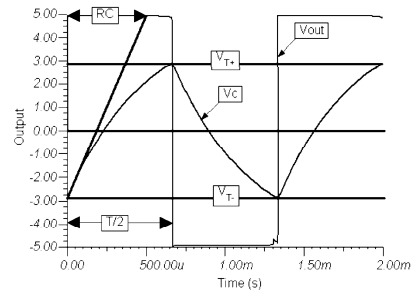
\includegraphics[width=6cm]{bilder/osziRechteckSignal.png}
		\columnbreak
		
		$V_{T+}=V_{outMAX}=\frac{R_2}{R_2+R_3}$\\
		$V_{T-}=V_{outMIN}=\frac{R_2}{R_2+R_3}$\\
		$V_c(t)=V_{T-}+\left(V_{outMAX}-V_{T-}\right)\left(1-e^{\frac{-t}{R_1\cdot
		C_1}}\right)$\\
		$f=\frac{1}{T}=\frac{1}{2R_1C_1 ln \frac{R_3+2R_2}{R3}}$\\
		wenn: $R2 = 0.86 \cdot R_3$ dann $ln\frac{R_3 +2 \cdot 0.86 \cdot R_3}{R_3}=ln
		\left( 2.72 \right) = 1$\\
		$\Longrightarrow f=\frac{1}{2\cdot R_1C_1}$
	\end{multicols}
\subsection{Dreieck Rechteck Generator}
	\begin{multicols}{3}
		\begin{center}
			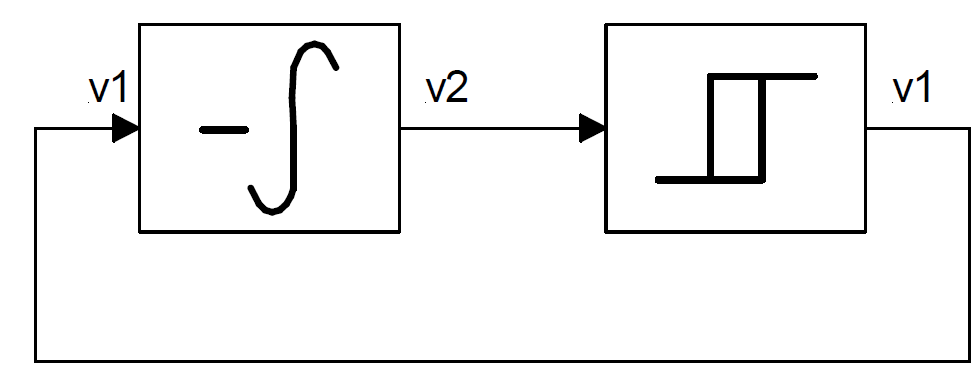
\includegraphics[width=3.5cm]{bilder/osziDreieckRechteckBlock.png}\\
		\end{center}
		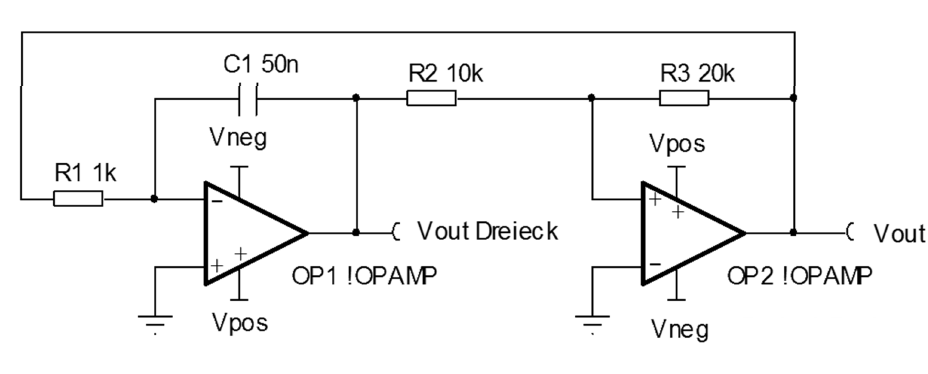
\includegraphics[width=6cm]{bilder/osziDreieckRechteck.png}
		\columnbreak
		
		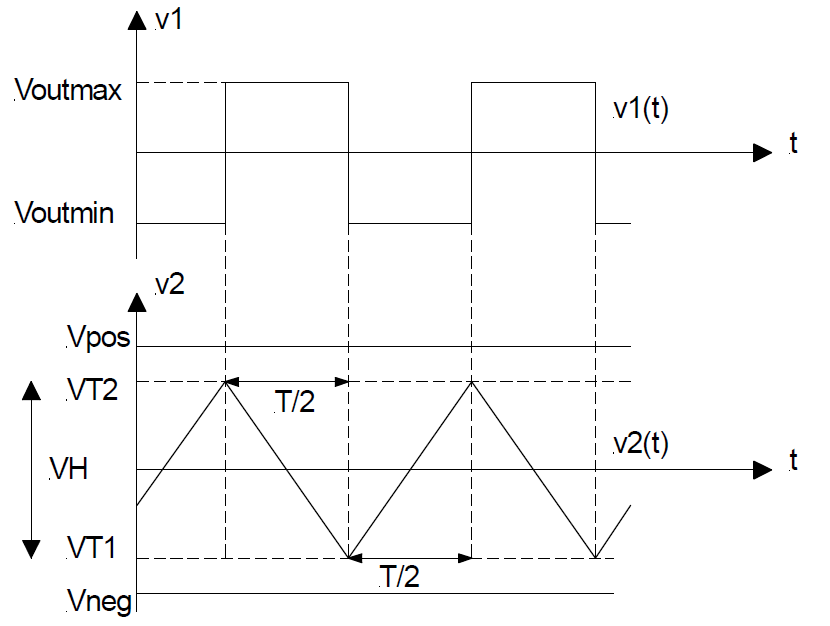
\includegraphics[width=6cm]{bilder/osziDreieckRechteckSignal.png}
		\columnbreak
			
		$V_2\left(t\right)=-\frac{1}{R_1C}\int V_1\left(t\right)dt+V_{2 Anfang}$\\
		$V_H=2\left|V_T\right|=\left(V_{outMAX}-V_{outMIN}\right)\frac{R_2}{R_3}$\\
		$T=\frac{2\cot V_H \cdot R_1C}{V_{outMAX}}$\\
	\end{multicols}
\subsection{Ringoszilatoren}
	\begin{multicols}{3}
	 	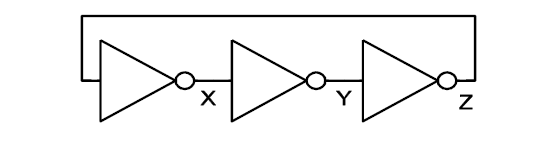
\includegraphics[width=6cm]{bilder/osziRing.png}	
		\columnbreak
		
		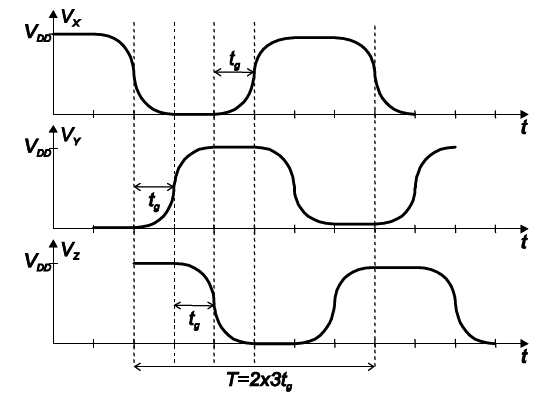
\includegraphics[width=6cm]{bilder/osziRingSignal.png}	
		\columnbreak
		
		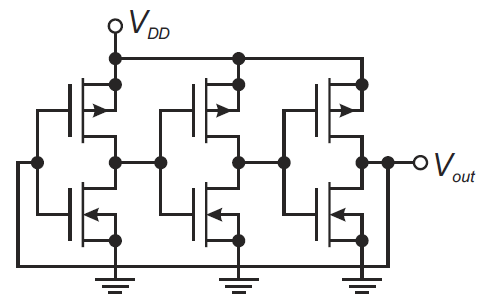
\includegraphics[width=6cm]{bilder/osziRingCMOS.png}
	\end{multicols}
\subsection{VCO (voltage controlled oscialltors)}
	\begin{multicols}{2}
		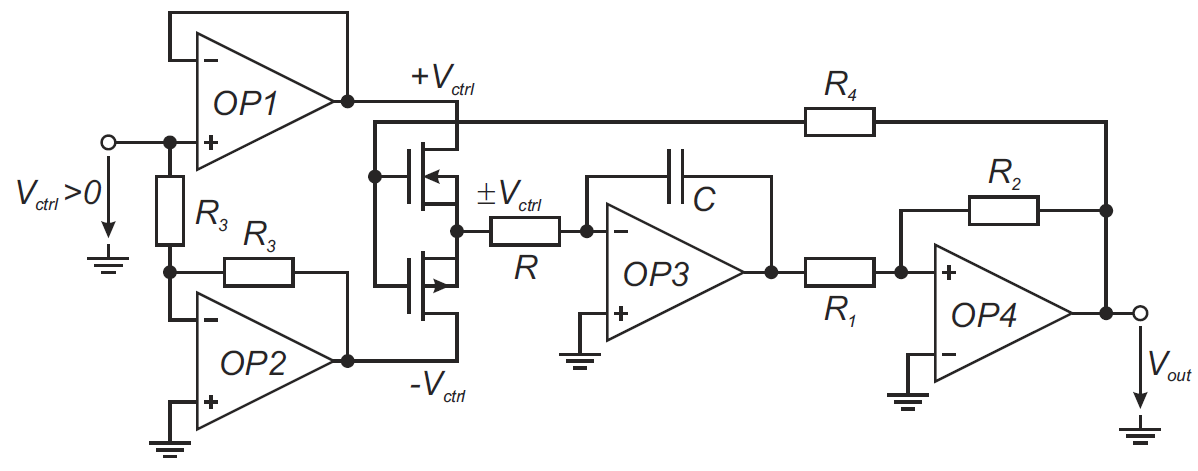
\includegraphics[width=9cm]{bilder/osciVCO.png}
		\columnbreak
		
		$OP4$ bildet mit $R_1$ und $R_2$ einen Schmitt-Trigger.\\
		$OP3$ bildet mit $R$ und $C$ ein Integrator.\\
		$f_{osc}=\frac{R_2}{4\cdot R_1}\cdot \frac{1}{RC}\cdot
		\frac{V_{ctrl}}{\left|V_{out}\right|}=K_{VCO}\cot V_{ctrl}$\\
	\end{multicols}
\subsection{LC-Oszillator}
	\begin{multicols}{3}
		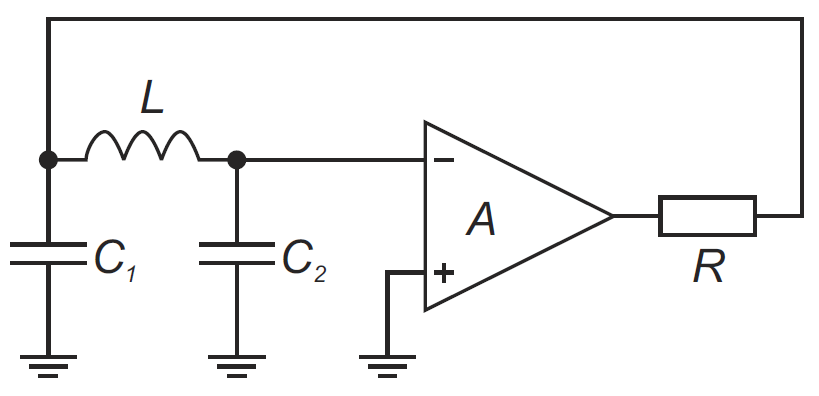
\includegraphics[width=6cm]{bilder/osziLC.png}\\
		Aufbau eine Colpitts-Oszillators
		\columnbreak
		
		$T\left(s\right)=\frac{-A}{1+sR\left(C_1+C_2\right)+s^2LC_2+s^3RLC_1C_2}$\\
		$s=j\omega$ und $\Im{T\left(j\omega\right)}=0$ ergeben $\omega_0$\\
		$\omega_0=\frac{1}{\sqrt{L\frac{C_1 C_2}{C_1+C_2}}}$\\
		\columnbreak
		
		Aus $T\left(j\omega\right)=1$ ergeben die Amplituden = und Anschwingbedignugnen
		$\geq$
		$A=\frac{C_2}{C_1}$ bzw. $A\geq\frac{C_2}{C_1}$
	\end{multicols}
\subsection{Quarz-Oszilator}
	\begin{multicols}{3}
		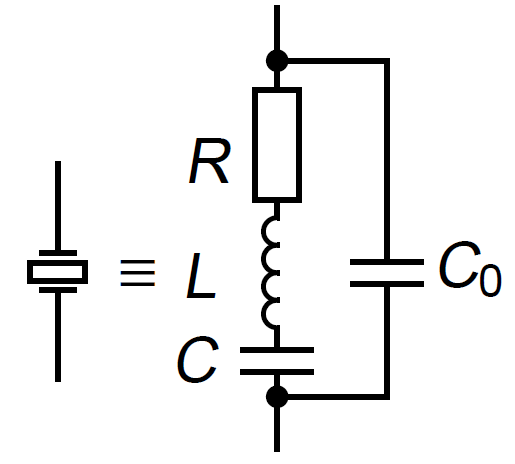
\includegraphics[width=3cm]{bilder/osziCrystal.png}
		\columnbreak
		
		$Z_{Xtal}\left(\omega\right)=\frac{\left(R+sL+\frac{1}{sC}\right)\frac{1}{sC_0}}{R+sL+\frac{1}{sC}+\frac{1}{sC_0}}$\\
		\\
		Wenn $R \ll \omega L$:\\
		$Z_{Xtal}\left(\omega\right)=\frac{s^2LC+1}{s\left(s^2LCC_0+C+C_0\right)}$\\
		\columnbreak
		
		f\"ur $Z\left(s\right)=jX\left(\omega\right)$:\\
		\\
		$X\left(\omega\right)=-\frac{1}{\omega C_0}\cdot \frac{\omega^2 -
		\omega_s^2}{\omega^2-\omega^2_P}$
	\end{multicols}